
\lecture{Measures Of Position}{measures-of-position}
\section{Measures Of Position}


\title{Measures Of Position}
\subtitle{Where are you?}

%\author{Kelly Black}
%\institute{Clarkson University}
\date{20 January 2012}

\begin{frame}
  \titlepage
\end{frame}

\begin{frame}
  \frametitle{Outline}
  \tableofcontents[pausesection,hideothersubsections,sectionstyle=show/hide]
\end{frame}


\subsection{Clicker Quiz}


\begin{frame}
  \frametitle{Clicker Quiz}

  \vfill
  Find the third quartile of the following data set:\\
  \begin{tabular}{llllll}
    28, & 17, & 12, & 20, & 21, & 18
  \end{tabular}

  \vfill

  \begin{tabular}{l@{\hspace{3em}}l@{\hspace{3em}}l}
    A: 17 & B: 19 & C: 21
  \end{tabular}

  \vfill

\end{frame}




\subsection{Percentiles}

\begin{frame}
  \frametitle{Percentiles}

  \begin{definition}
    The P\textsuperscript{th} percentile is the data point for which P\%
    of the numbers are smaller than it.
  \end{definition}

\end{frame}

\begin{frame}
  \frametitle{Percentiles}

%  \begin{eqnarray*}
%    \begin{array}{lllll}
%      x_1 & x_2 & x_3 & \cdots & x_n \\
%    \end{array}
%  \end{eqnarray*}

  \newcount\xnum
  \newcount\xnumpos
  \only<1>
  {
    \begin{picture}(500,100)(0,0)
      \multiput(10,90)(20, 0){15}{\line(1,0){15}}
      \xnum=1
      \xnumpos=12
      \loop
      \put(\xnumpos,95){$x_{{\the\xnum}}$}
      \advance\xnumpos by 20
      \ifnum\xnum < 15 \advance\xnum by 1
      \repeat
    \end{picture}
  }

  \only<2>
  {
    \begin{picture}(310,100)(0,0)
      \multiput(10,90)(20, 0){15}{\line(1,0){15}}
      \xnum=1
      \xnumpos=12
      \loop
      \put(\xnumpos,95){$x_{{\the\xnum}}$}
      \advance\xnumpos by 20
      \ifnum\xnum < 15 \advance\xnum by 1
      \repeat
      \put(10,0){\line(0,1){80}}
      \put(310,0){\line(0,1){80}}
      \put(110,20){\vector(-1,0){100}}
      \put(210,20){\vector( 1,0){100}}
      \put(120,15){Width=n Items}
    \end{picture}
  }

  \only<3>
  {
    \begin{picture}(310,100)(0,0)
      \multiput(10,90)(20, 0){15}{\line(1,0){15}}
      \xnum=1
      \xnumpos=12
      \loop
      \put(\xnumpos,95){$x_{{\the\xnum}}$}
      \advance\xnumpos by 20
      \ifnum\xnum < 15 \advance\xnum by 1
      \repeat
      \put(10,0){\line(0,1){80}}
      \put(310,0){\line(0,1){80}}
      \put(110,20){\vector(-1,0){100}}
      \put(210,20){\vector( 1,0){100}}
      \put(120,15){Width=n Items}

      \put(250,50){\line(0,1){40}}
      \put(80,60){\vector(-1,0){70}}
      \put(180,60){\vector( 1,0){70}}
      \put(85,55){P Percent of Width}

    \end{picture}
  }

  \vfill
  
\end{frame}

\begin{frame}
  \frametitle{Percentiles}

    \begin{picture}(310,100)(0,0)
      \multiput(10,90)(20, 0){15}{\line(1,0){15}}
      \xnum=1
      \xnumpos=12
      \loop
      \put(\xnumpos,95){$x_{{\the\xnum}}$}
      \advance\xnumpos by 20
      \ifnum\xnum < 15 \advance\xnum by 1
      \repeat
      \put(10,0){\line(0,1){80}}
      \put(310,0){\line(0,1){80}}
      \put(110,20){\vector(-1,0){100}}
      \put(210,20){\vector( 1,0){100}}
      \put(120,15){Width=n Items}

      \put(250,50){\line(0,1){40}}
      \put(70,60){\vector(-1,0){60}}
      \put(190,60){\vector( 1,0){60}}
      \put(75,55){j/n items = k\textsuperscript{th} percent}

    \end{picture}


    \begin{eqnarray*}
      P & = & \frac{k}{100}, \\
      \frac{j}{n} & = & \frac{k}{100}, \\
      \Rightarrow j & = & \frac{nk}{100}.
    \end{eqnarray*}

\end{frame}

\begin{frame}
  \frametitle{Example}

  \vfill 

  Find the 85\textsuperscript{th} percentile for the following data:

  \vfill

  \only<1>
  {
    89, 85, 97 106, 94, 100, 92, 120, 92, 97, 89, 90, 103, 86, 106, 112, 100, 92, 84,
    97, 103, 91, 104, 91, 104
  }

  \only<2>
  {
    Sort it: \\
    84, 85, 86, 89, 89, 90, 91, 91, 92, 92, 92, 94, 97, 97, 97, 100,
    100, 103, 103, 104, 104, 106, 106, 112, 120
  }

  \only<3>
  {
    Sort it: \\
    84, 85, 86, 89, 89, 90, 91, 91, 92, 92, 92, 94, 97, 97, 97, 100,
    100, 103, 103, 104, \underline{104}, \underline{106}, 106, 112, 120
  }


  \vfill

  (There are 25 data points.)

  \vfill

\end{frame}

\begin{frame}
  \frametitle{Clicker Quiz}

  \vfill

  Find the 30\textsuperscript{th} percentile for the following data:

  185, 196, 214, 199, 199, 204


  \vfill

  \begin{tabular}{l@{\hspace{3em}}l@{\hspace{3em}}l}
    A: 198 & B: 198 $\frac{2}{5}$ & C: 199
  \end{tabular}



\end{frame}

\subsection{Box Plots}

\begin{frame}
  \frametitle{Box Plots}

  \vfill 

  Find the five point summary for the following data:

  \vfill

  \only<1>
  {
    89, 85, 97 106, 94, 100, 92, 120, 92, 97, 89, 90, 103, 86, 106, 112, 100, 92, 84,
    97, 103, 91, 104, 91, 104

    \vfill
  }

  \only<2>
  {
    Sort it: \\
    84, 85, 86, 89, 89, 90, 91, 91, 92, 92, 92, 94, 97, 97, 97, 100,
    100, 103, 103, 104, 104, 106, 106, 112, 120

    Five point summary: \\
    \begin{tabular}{lllll}
     Min. & 1st Qu. & Median    & 3rd Qu. &   Max. \\
     84   & 91      & 97        & 103     & 120
    \end{tabular}


  }

  \vfill

\end{frame}


\begin{frame}
  \frametitle{Box Plots}

    Five point summary: \\
    \begin{tabular}{lllll}
     Min. & 1st Qu. & Median    & 3rd Qu. &   Max. \\
     84   & 91      & 97        & 103     & 120
    \end{tabular}

    \begin{center}
      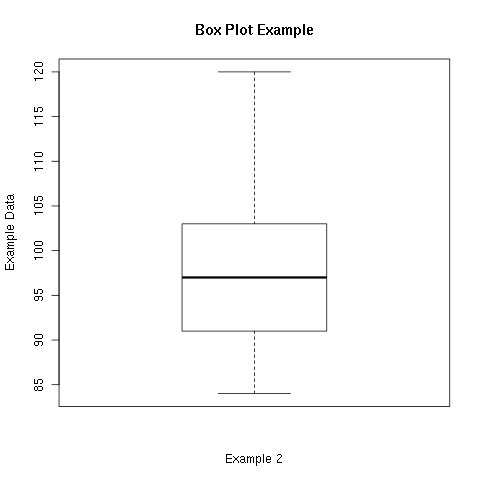
\includegraphics[width=6cm]{img/boxplotExample1}
    \end{center}

\end{frame}



\begin{frame}
  \frametitle{Z-Score}

  \begin{definition}
    Given a set of data,
    \begin{eqnarray*}
      x_1,~x_2,~x_3,\ldots,x_n,
    \end{eqnarray*}
    with sample mean $\bar{x}$ and standard deviation $s$ the
    $z$-score for a number, $x$, is
    \begin{eqnarray*}
      z & = & \frac{x-\bar{x}}{s}.
    \end{eqnarray*}
  \end{definition}

\end{frame}


% LocalWords:  Clarkson pausesection hideallsubsections
